\part{行为的发育和出现}
\markboth{总论}{总论}

\begin{figure}[htbp]
	\centering
	\includegraphics[width=0.95\linewidth]{chap45/fig_45_0}
	\caption{小鼠视网膜中单一类型视网膜神经节细胞的转基因标记。
		颜色代表视网膜的深度,表面的轴突为蓝色,最深的树突为红色。
		不完全了解的引导机制导致\textit{JamB 视网膜神经节细胞}树突“指向”腹侧,从而导致它们对腹侧运动的优先反应。
		\textit{JamB 视网膜神经节细胞}轴突被引导到视神经,通过视神经到达大脑的其余部分。}
	\label{fig:45_0}
\end{figure}


成熟的神经系统控制无数的行为(我们的思想、感知、决策、情绪),而行为则取决于大脑和脊髓中数十亿神经元之间突触连接的精确模式。
这些连接在胚胎期和出生后早期形成,但可以在整个生命过程中被重塑。
在本节中,我们将描述神经系统是如何发育和成熟的。


发育神经生物学的历史悠久而辉煌。大约 150 年前,\textit{圣地亚哥$\cdot$拉蒙$\cdot$卡哈尔}对神经系统的结构和组织进行了一系列全面的解剖学研究,然后开始探索其发育。
他唯一可用的方法是对固定组织进行光学显微镜分析,但从他的观察中,他推断出许多仍然被认为是正确的发育原理。
在 20 世纪上半叶,其他解剖学家追随他的脚步。
随着新方法的出现,发育加快了,首先是电生理学和电子显微镜,最近是分子生物学,遗传学和实时成像。
我们现在对决定神经细胞如何获得其身份、如何将轴突延伸到靶细胞以及这些轴突在到达目的地后如何选择合适的突触伙伴分子有了大量的了解。


将构成神经发育的众多步骤分为三个时期是有效的,尽管它们在时间上有一定程度的重叠,但在概念上是不同的。
首先,从胚胎发生的最早阶段开始,导致神经元和神经胶质的产生和分化。
人们可以把这个时期看作是致力于生产\textit{组装神经回路组件}的时期:硬件。
这些步骤取决于特定基因在特定时间和地点的表达。
控制这些时空模式的一些分子是转录因子,它们在\textit{脱氧核糖核酸}水平上起作用以调节基因表达。
它们在分化细胞内起作用,因此被称为细胞自主因子。
其他因子被称为细胞非自主因子,包括细胞表面和其他细胞产生的分泌分子。
它们通过与分化细胞上的受体结合并产生信号来调节细胞自主转录程序活性。
这些内在因子和外在因子的相互作用对于每个神经细胞的正确分化至关重要。


第二个时期包括神经元连接的步骤:将其躯体迁移到适当的位置,将轴突引导到其靶标,并形成突触连接。
神经连接问题的复杂性是惊人的,比如许多神经元类型的轴突必须导航,通常是长距离导航,然后在一百个或更多\textit{突触后电位}伴侣中进行选择。
尽管如此,取得了令人鼓舞的进展。
一个主要因素是通过分析\textit{果蝇}和\textit{秀丽隐杆线虫}等简单且可遗传的生物来解决这个问题的能力。
事实证明,许多控制神经系统形成的关键分子在经过数百万年进化分离的生物体中都是保守的。
因此,尽管动物形式多样,但控制身体计划和神经连接的发育程序在整个系统发育过程中都是保守的。


在第三个时期,由基因决定的连接模式(硬件)是由活动和经验(软件)塑造的。
不幸的是,对于研究人员来说,哺乳动物的这些步骤与无脊椎动物和低等脊椎动物的共享程度非常有限。
一只刚孵出的鸟或苍蝇在行为上与成年的自己没有明显的不同,但没有人可以这样说一个人。
这在很大程度上是因为我们的神经系统在出生时有点粗糙。
制定其基本计划的硬连线回路在出生后的很长一段时间内通过经验和神经活动进行修改。
这样,每个人的经历都可以在他的神经系统上留下不可磨灭的印记,学习可以增强大脑的认知能力。
这些过程在所有哺乳动物中都起作用,神经科学家现在使用小鼠来探索它们背后的机制,但它们在人类中尤为突出和持久。
这可能是经验可以塑造人类神经系统的长期时间是使其能力在所有物种中独一无二且最重要的单一因素。


随着我们对发育理解的增加,它越来越多地为神经病学和精神病学提供信息。
许多调节前两个时期的基因现在被认为是某些神经退行性疾病和行为障碍的\textit{敏感因子},甚至是其原因。
因此,对神经发育的研究开始为神经疾病病因提供见解,并提出在疾病或创伤性损伤后恢复神经连接和功能的合理策略。
最近,随着我们了解经验依赖性重塑背后的细胞和分子变化,例如,我们可以希望了解,在生命早期如此明显的可塑性是如何在成年人身上被利用的,以改善受伤、中风或神经退行性疾病后的康复治疗。
此外,越来越多的理由相信,某些行为障碍(例如孤独症或精神分裂症)可能部分是由于出生后早期神经回路的经验依赖性调节缺陷所致。


第七部分按顺序总结了这些时期。
从神经发育的早期阶段开始,我们专注于控制神经细胞多样性和存活、引导轴突和调节突触形成的因素。
然后,我们解释了如何与环境互相影响,包括社会的和身体的的互相影响,如何改变或巩固早期发育过程中形成的神经联系。
最后,我们研究了成年人如何利用发育过程,以及类固醇激素等因素如何塑造大脑,影响性和性别认同。
第九部分的第~\ref{chap:chap64}~章介绍了随着大脑老化而发生的最后几步变化。



\chapter{神经系统的塑造} \label{chap:chap45}

在脊椎动物神经系统的发育过程中会产生大量的神经元和神经胶质细胞。
不同类型的神经元在离散的解剖位置发育,获得不同的形态学形式,并与特定的靶细胞群建立联系。
它们的多样性远远超过身体任何其他器官中的细胞。
例如,视网膜有几十种中间神经元,脊髓有一百多种运动神经元。
目前,哺乳动物中枢神经系统中神经元类型的真实数量仍然未知,但肯定超过一千种。
神经胶质类型的数量就更不清楚了。
直到最近,在被认为是相当同质的星形胶质细胞和少突胶质细胞类别中发现了意想不到的异质性。


神经元类型的多样性是哺乳动物神经系统令人印象深刻的计算特性的基础。
然而,正如我们在本章和后续章节中所描述的那样,驱动神经系统分化的发育原则是从用于指导其他组织发育的原则中借鉴的。
从某种意义上说,神经系统的发育仅仅代表了一个复杂的例子,说明了贯穿于所有发育生物学的基本挑战:如何将单个受精卵细胞转化为成熟生物体所特有的高度分化的细胞类型。
只有在后期阶段,当神经元形成复杂的回路并且经验改变它们的连接时,神经发育的原则才会与其他器官的原则不同。


早期发育原则不仅在生物组织之间是保守的,而且在物种和\textit{门}之间也是保守的。
事实上,我们对脊椎动物神经发育的细胞基础和分子基础的了解大部分来自所谓简单生物的遗传研究,最著名的是\textit{黑腹果蝇}和\textit{秀丽隐杆线虫}。
然而,由于研究神经发育的主要目标是解释神经系统的组装如何成为人类行为和大脑障碍的基础,因此我们对神经系统发育规则和原则的描述主要集中在脊椎动物身上。



\section{神经管起源于外胚层}

脊椎动物胚胎来自受精卵。
如图~\ref{fig:45_1}A~所示,细胞分裂最初形成一个称为\textit{桑葚胚}的细胞球,然后空心形成\textit{囊胚}。
接下来,折叠和生长产生\textit{原肠胚},这是一种具有极性(背侧-腹侧、前侧-后侧)和三层细胞(内胚层、中胚层和外胚层)的结构。


\begin{figure}[htbp]
	\centering
	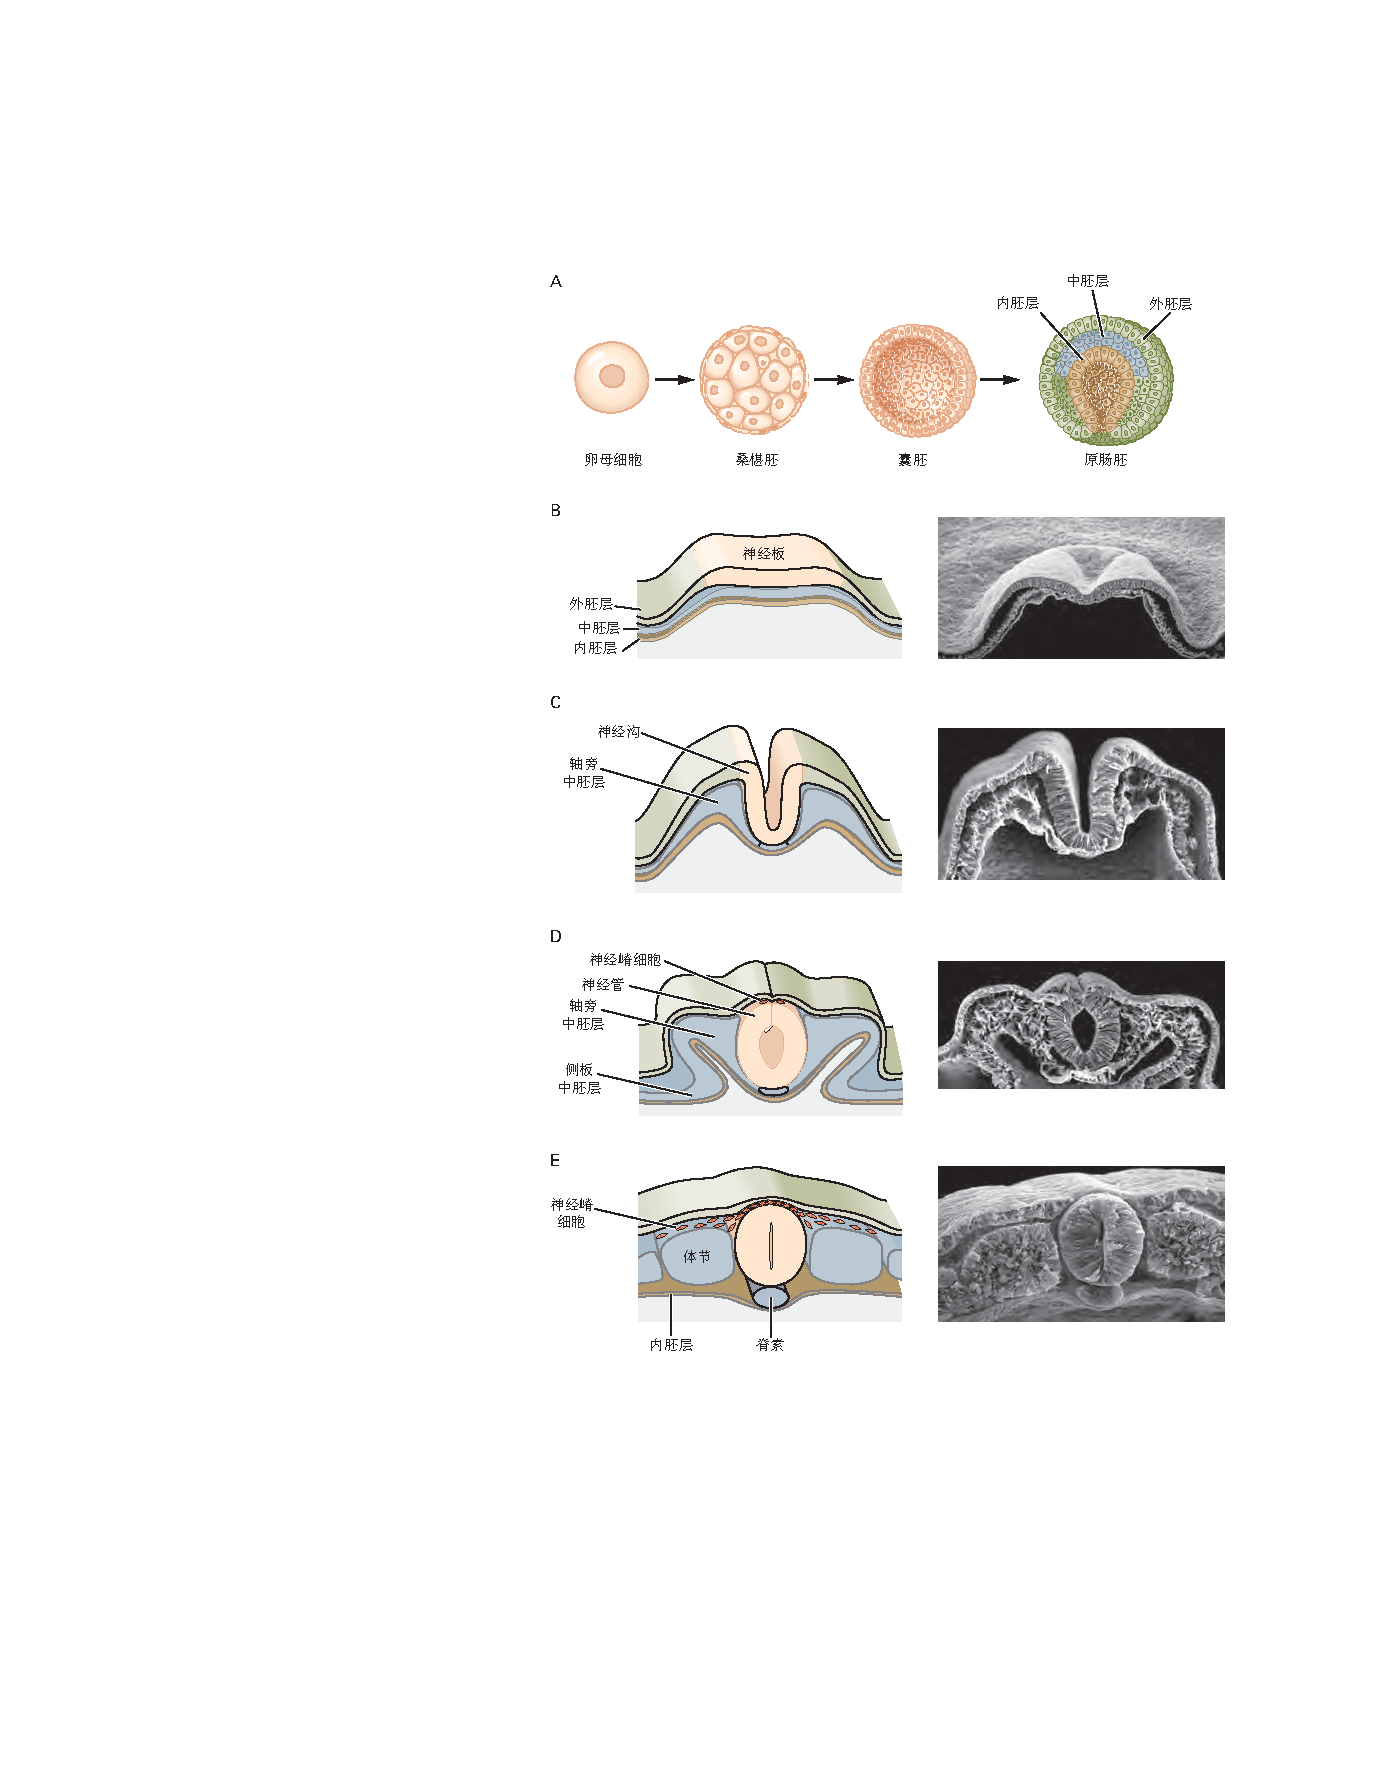
\includegraphics[width=0.81\linewidth]{chap45/fig_45_1}
	\caption{\textit{神经板}折叠形成\textit{神经管}。
		% 卵母细胞是在卵子发生过程中进行减数分裂的卵原细胞。分为初级卵母细胞、次级卵母细胞和成熟的卵母细胞。 卵母细胞的最终形成产物就是卵细胞,也就是我们日常所说的卵子。
		A. \textit{卵子}受精后,细胞分裂依次产生\textit{桑葚胚}、\textit{囊胚}和\textit{原肠胚}。
		三个生殖细胞层(外胚层、中胚层和内胚层)在原肠胚形成过程中形成。
		B. 一条外胚层变成\textit{神经板},这是\textit{中枢神经系统}和\textit{周围神经系统}的前身。
		C. 神经板在中线处弯曲形成\textit{神经沟}。
		D. 背侧神经折叠的闭合形成\textit{神经管}。
		E. 神经管位于\textit{脊索}上方,两侧是\textit{体节},体节是产生肌肉和软骨的卵圆形中胚层细胞群。
		\textit{神经管}和覆盖的\textit{外胚层}交界处的细胞被放在一边,成为\textit{神经嵴}。}
	\label{fig:45_1}
\end{figure}


\textit{内胚层}是最里面的胚层,后来产生肠道、肺、胰腺和肝脏。
\textit{中胚层}是产生肌肉、结缔组织和大部分血管系统的中间胚层。
\textit{外胚层}是最外层。
如图~\ref{fig:45_1}B~所示,大部分外胚层产生\textit{皮肤},但有一条狭窄的中央带向外延伸形成\textit{神经板}。
中枢神经系统和周围神经系统是从神经板产生的。


如图~\ref{fig:45_1}C,D~所示,神经板形成后不久,它开始内陷,形成\textit{神经沟}。
然后褶皱加深并最终与外胚层的其余部分分离,形成\textit{神经管},这一过程称为\textit{神经胚形成}。
神经管的\textit{尾侧}区域形成\textit{脊髓},而\textit{嘴侧}区域形成\textit{大脑}。
如图~\ref{fig:45_1}E~所示,随着神经管的闭合,与外胚层连接处的细胞被分离出来,形成\textit{神经嵴},最终形成自动神经系统和感觉神经系统,以及几种非神经细胞类型。



\section{分泌信号促进神经细胞命运}

与其他器官一样,神经系统的出现是一个复杂分子程序的顶峰,该程序涉及特定基因的紧密协调表达。
对于神经系统,第一步是从外胚层的限制区域形成神经板。
这一步反映了外胚层细胞必须做出的早期选择的结果:是成为神经细胞还是\textit{表皮细胞}。
近 100 年来,这一决定一直是人们深入研究的主题。


这项工作的大部分集中在寻找控制外胚层细胞命运的信号。
我们现在知道,两大类蛋白质共同作用,促进外胚层细胞分化为神经细胞。
第一种是\textit{诱导因子},即附近细胞分泌的信号分子。
其中一些因子可自由扩散并在一定距离内发挥作用,但其他因子则被束缚在细胞表面并在局部发挥作用。
第二种是使细胞能够对诱导因子作出反应的表面受体。
这些受体的激活会触发编码细胞内蛋白质(转录因子、酶和细胞骨架蛋白)的基因的表达,从而推动外胚层细胞沿着通路成为神经细胞。


细胞对诱导信号作出反应的能力,称为其感受态,取决于它表达的受体、转导分子和转录因子的确切库。
因此,细胞的命运不仅取决于它所暴露的信号(这是它在胚胎中何时何地发现自己的结果),而且还取决于它先前发育史所表达的\textit{基因谱}。
我们将在后续章节中看到,局部感应信号和固有细胞反应的相互作用在神经发育的几乎每一步中都是明显的。



\subsection{神经板的发育是由组织区的信号诱导的}

发现特定信号负责触发神经板形成是理解神经系统模式机制的第一个重大进展。
1924 年,\textit{汉斯$\cdot$斯佩曼}和\textit{希尔德$\cdot$曼戈尔德}发现,神经板与未定型外胚层的分化取决于一组被称为\textit{组织区}的特殊细胞分泌信号。


他们的实验包括将小块组织从一个两栖动物胚胎移植到另一个胚胎。
最有说服力的是将胚孔的\textit{背唇}从正常的\textit{背侧}位置移植到宿主胚胎的\textit{腹侧},胚孔的背唇注定要形成背侧中胚层。
如图~\ref{fig:45_2}~所示,背唇位于背外胚层下方,该区域通常会产生背表皮,包括神经板。
他们将有色胚胎的组织移植到无色素的宿主中,使他们能够区分供体细胞和宿主细胞的位置和命运。


\begin{figure}[htbp]
	\centering
	\includegraphics[width=0.62\linewidth]{chap45/fig_45_2}
	\caption{来自组织区的信号诱导第二个神经管。
		左图:在正常青蛙中,来自组织区(背胚孔唇)的胚胎细胞分布在\textit{脊索}、底板和\textit{体节}上。
		右图:\textit{斯佩曼}和\textit{曼戈尔德}将原肠胚早期胚胎的\textit{背侧}胚孔唇移植到宿主胚胎的一个区域,该区域通常会产生\textit{腹侧}表皮。
		来自移植细胞的信号诱导第二个胚胎轴,其中包括一个几乎完整的神经管。
		供体组织来自有色素的胚胎,而宿主组织没有色素,因此可以通过颜色监测移植细胞的命运。
		移植细胞本身仅对宿主胚胎的脊索、底板和体节有贡献。
		随着胚胎的成熟,次级神经管发育成一个完整的神经系统。
		如图~\ref{fig:45_3}~所示,在显微照片中显示的非洲爪蟾胚胎中,第二个神经轴是通过注射\textit{骨形态发生蛋白}拮抗剂诱导的,实际上替代了组织者信号。
		初级神经轴也很明显。}
	\label{fig:45_2}
\end{figure}


\begin{figure}[htbp]
	\centering
	\includegraphics[width=1.0\linewidth]{chap45/fig_45_3}
	\caption{\textit{骨形态发生蛋白}信号的抑制启动神经诱导。
		A. 在\textit{爪蟾}蛙胚胎中,来自组织区(红线)的信号通过外胚层传播以诱导神经组织。
		超出组织信号范围的外胚层组织产生\textit{表皮}。
		B. 从\textit{组织区}分泌的\textit{骨形态发生蛋白}抑制剂(包括\textit{脊索发生素}、\textit{头蛋白}、\textit{卵泡抑素})与\textit{骨形态发生蛋白}结合并阻断外胚层细胞获得表皮命运的能力,从而促进\textit{神经特性}。
		C. 外胚层细胞根据是否存在\textit{骨形态发生蛋白}信号获得\textit{神经特性}或表皮特性。
		当外胚层细胞聚集体暴露于\textit{骨形态发生蛋白}信号时,它们会分化为表皮组织。
		当\textit{骨形态发生蛋白}信号被阻断时,无论是通过将外胚层组织分离成单个细胞,还是通过将\textit{骨形态发生蛋白}抑制剂添加到外胚层细胞聚集体中,细胞都会分化为神经组织。}
	\label{fig:45_3}
\end{figure}


\textit{斯佩曼}和\textit{曼戈尔德}发现,从胚孔背唇移植的细胞遵循它们的正常发育程序,产生中线中胚层组织,如体节和脊索。
但是移植的细胞也引起了宿主胚胎相邻的腹外胚层细胞命运的显著变化。
如图~\ref{fig:45_2}~所示,宿主外胚层细胞被诱导形成几乎完整的神经系统副本。
因此,他们称供体组织为\textit{组织者}。
\textit{斯佩曼}和和\textit{曼戈尔德}继续证明胚孔的背唇是唯一具有这种“组织”作用的组织。


这些开创性研究还表明,“诱导”在神经发育中起着至关重要的作用。
诱导是一种过程,通过该过程,一个组织的细胞在两个接近的区域指导相邻细胞的发育。
重要的是它提供了一种机制,来自一个组织的信号可以通过该机制导致第二个组织的细分。
在这种情况下,中胚层诱导外胚层的一部分变成神经板,最终变成神经系统,而其余部分继续变成上皮,最后变成皮肤。
由此形成的新毗邻原则上可以为随后一连串的归纳和细分奠定基础。
事实上,我们将看到,神经管模式的许多方面都依赖于局部组织中心分泌的信号,这些信号的作用原理上与经典的组织者区相似。



\subsection{神经诱导是由肽生长因子及其抑制剂介导的}

在\textit{斯佩曼}和\textit{曼戈尔德}的开创性研究之后的几十年里,神经诱导剂的鉴定构成了发育生物学的圣杯。
直到 1980 年代,当分子生物学的出现和早期神经组织更好的标记物的可用性导致我们对神经诱导及其化学介质的理解取得了突破时,这项研究才取得了一些成功。


如图~\ref{fig:45_3}A~所示,第一个进展来自一个简单的发现:当早期外胚层分离成单个分离细胞时,有效地阻止了细胞间信号传导,细胞在没有添加因子的情况下很容易获得神经特性。
这一发现的令人惊讶的含义是,外胚层细胞的“默认”命运是神经分化,而这种命运是通过外胚层细胞之间的信号传递来阻止的。
在这个模型中,长期以来备受追捧的“\textit{诱导剂}”实际上是一种“\textit{去阻遏物}”:它阻止外胚层抑制神经命运。


这些想法立即引发了两个进一步的问题。
什么外胚层信号抑制神经分化,\textit{组织者细胞}提供什么来克服阻遏物的影响?
青蛙和小鸡的神经诱导研究现已为这些问题提供了答案。


在没有来自\textit{组织者细胞}的信号的情况下,外胚层细胞合成并分泌\textit{骨形态发生蛋白},这是\textit{转化生长因子$\beta$}相关蛋白大家族的成员。
如图~\ref{fig:43_3}B~所示,\textit{骨形态发生蛋白}通过外胚层细胞上的丝氨酸/苏氨酸激酶类受体发挥作用,抑制神经分化的潜力并促进表皮分化。
\textit{骨形态发生蛋白}作为神经抑制因子作用的关键证据来自实验,在实验中,发现\textit{骨形态发生蛋白}受体的截短形式会触发非洲爪蟾胚胎中的神经组织分化。
相反,如图~\ref{fig:45_3}C~所示,外胚层细胞暴露于\textit{骨形态发生蛋白}信号转导促进分化为表皮细胞。


\textit{骨形态发生蛋白}作为神经元分化抑制因子的鉴定反过来表明,\textit{组织者细胞}可能通过分泌拮抗\textit{骨形态发生蛋白}信号传导的因子来诱导外胚层细胞的神经分化。
对这一想法的直接支持来自发现组织者区的细胞表达许多作为\textit{骨形态发生蛋白}拮抗剂的分泌蛋白。
这些蛋白质包括\textit{头蛋白}、腱蛋白、卵泡抑素蛋白,甚至一些变异的\textit{骨形态发生蛋白}。
如图~\ref{fig:45_3}B~所示,这些蛋白质中的每一种都具有诱导外胚层细胞分化为神经组织的能力。
因此,没有单一的神经诱导剂。
事实上,诱导需要多种蛋白质,正如后来发现的那样,外胚层细胞暴露于\textit{成纤维细胞生长因子}也是神经分化的必要步骤。


总之,这些研究为神经诱导的细胞现象提供了分子解释。
尽管该通路的许多细节仍有待阐明,并且物种之间的一些机制差异仍然令人费解,但在\textit{斯佩曼}和\textit{曼戈尔德}发现\textit{组织者细胞}近一个世纪后,神经发育的关键一章现在已经得出了令人满意的结论。



\section{神经管的头尾模式涉及信号梯度和二级组织中心}

一旦神经板的细胞被诱导,它们就开始获得区域特征,这些区域特征标志着将神经系统划分为前脑、中脑、后脑和脊髓等区域的第一步。
这种细分由一系列分泌的诱导因子指导,并遵循着神经诱导的相同基本原理。
神经管不同区域的神经板细胞通过表达不同的转录因子来响应这些感应信号,这些转录因子逐渐限制每个局部区域中细胞的发育潜能。
这样,不同位置的神经元就获得了功能差异。
信号沿神经管的头尾轴和背腹轴发生。
我们首先描述头尾模式,然后返回到背腹模式。



\subsection{神经管在发育早期就区域化了}

神经管形成后,细胞分裂迅速,但增殖速度并不均匀。
神经上皮细胞的各个区域以不同的速度扩张,并开始形成成熟中枢神经系统的特殊部分。
神经管头端区域细胞增殖率的差异导致三种脑小泡的形成:
如图~\ref{fig:45_4}A~所示,前脑囊泡、中脑囊泡和后脑(或菱脑)囊泡。


\begin{figure}[htbp]
	\centering
	\includegraphics[width=1.0\linewidth]{chap45/fig_45_4}
	\caption{神经管发育的连续阶段。
		A. 在神经管发育的早期阶段,有三个脑泡,它们将形成\textit{前脑}、\textit{中脑}和\textit{菱脑}(后脑)。
		B. 前脑和菱脑内的进一步分裂产生额外的囊泡。
		前脑分裂形成端脑和间脑,菱脑分裂形成后脑和髓脑。
		C. 五囊泡阶段鸡胚神经管的俯视图。
		D. 神经管在小泡之间的边界处弯曲,形成头曲、脑桥曲和颈曲。}
	\label{fig:45_4}
\end{figure}


在这个早期的三囊泡阶段,神经管弯曲两次:
一次在颈曲,即脊髓和后脑的交界处,一次在头曲,即后脑和中脑的交界处。
如图~\ref{fig:45_4}D~所示,第三个弯曲是\textit{桥曲},形成较晚,再之后颈屈曲伸直并变得不明显。
头曲在整个发育过程中保持突出,它的持续存在是前脑纵轴方向偏离脑干和脊髓方向的原因。


如图~\ref{fig:45_4}B、C~所示,随着神经管的发育,两个初级胚胎小泡进一步分裂,从而形成五个小泡。
前脑囊泡分裂形成端脑,端脑会形成皮层、海马体和基底神经节,间脑会形成丘脑、下丘脑和视网膜。
中脑不再进一步分裂,形成下丘和上丘以及其他中脑结构。
后脑囊泡分裂形成后脑,后脑会形成脑桥和小脑,以及中脑会产生延髓。
这些部分与脊髓一起构成了成熟中枢神经系统的主要功能区域(见第~\ref{chap:chap4}~章)。
神经管逐渐细分为这些功能域是受各种分泌信号的调节。



\subsection{来自中胚层和内胚层的信号定义了神经板的头尾模式}

最初认为,按照\textit{斯佩曼}和\textit{曼戈尔德}的定义,\textit{组织者细胞}的特征是一致的,因此诱导了最初一致的神经板。
然而,随后的研究表明,\textit{组织者细胞}是区域性的,并且几乎在感应开始时就分泌启动神经板头尾模式的因子。
一类重要的因子包括\textit{无翅型乳腺瘤病毒整合位点家族}蛋白(基于其创始家族成员果蝇 Wingless 蛋白和哺乳动物 Int1 原癌基因蛋白的首字母缩写词)。
其他包括视黄酸和\textit{成纤维细胞生长因子}。
它们由\textit{组织者细胞}的中胚层细胞以及附近的近轴中胚层产生。


\textit{无翅型乳腺瘤病毒整合位点家族}信号活动的净水平在神经板的嘴侧水平较低,并在尾端方向逐渐增加。
这种活性梯度的出现是因为与神经板尾部区域相邻的中胚层表达高水平的\textit{无翅型乳腺瘤病毒整合位点家族}。
神经板延髓区域下方的组织加强了这种梯度,是抑制\textit{无翅型乳腺瘤病毒整合位点家族}信号的分泌蛋白来源,就像\textit{骨形态发生蛋白}抑制剂在早期阶段减弱\textit{骨形态发生蛋白}信号一样。
因此,如图~\ref{fig:45_5}A~所示,沿着神经板逐渐靠近尾部位置的细胞暴露于越来越高水平的\textit{无翅型乳腺瘤病毒整合位点家族}活性,并获得更多的尾部区域特征,跨越从前脑到中脑再到后脑,最后到脊髓的整个范围。
这些结果表明,前部特征是神经组织的“默认”状态,\textit{无翅型乳腺瘤病毒整合位点家族}等信号强加了后部特征。
实际上,当通过应用\textit{骨形态发生蛋白}抑制剂诱导外胚层细胞成为神经细胞时,它们会分化为具有前部结构特征的细胞。


\begin{figure}[htbp]
	\centering
	\includegraphics[width=1.0\linewidth]{chap45/fig_45_5}
	\caption{早期前后模式信号建立不同的转录因子域并定义中脑-后脑边界区域的位置。
		A. 神经板的前后模式是通过将神经细胞暴露于\textit{无翅型乳腺瘤病毒整合位点家族}信号梯度来建立的。
		神经板的前(A)区域暴露于内胚层分泌的\textit{无翅型乳腺瘤病毒整合位点家族}抑制剂,因此仅感知低水平的\textit{无翅型乳腺瘤病毒整合位点家族}活性。
		神经板的更多靠后(P)区域逐渐暴露于来自近轴中胚层的高水平\textit{无翅型乳腺瘤病毒整合位点家族}信号和较低水平的\textit{无翅型乳腺瘤病毒整合位点家族}抑制剂。
		B. 为了响应此\textit{无翅型乳腺瘤病毒整合位点家族}信号梯度和其他信号,神经板前部和后部区域的细胞开始表达不同的转录因子:前部水平的 Otx2 和更后部水平的 Gbx2。
		这两个转录因子结构域的交叉点标志着\textit{中脑和后脑边界}区域,其中表达了\textit{齿状基因片段}转录因子。
		然后神经管形成\textit{中脑和后脑边界}前后的部分。
		C. 来自峡部\textit{组织者细胞}的\textit{成纤维细胞生长因子}信号与来自腹侧中线的\textit{音猬因子}信号协同作用,以指定多巴胺能和\textit{5-羟色氨}能神经元的身份和位置。
		这两类神经元的不同命运源于 Otx2 在中脑和 Gbx2 在后脑中的表达\cite{wurst2001neural}。}
	\label{fig:45_5}
\end{figure}



\subsection{来自神经管内组织中心的信号会影响前脑、中脑和后脑}

中胚层和内胚层组织对头尾神经模式的早期影响通过来自神经管本身的特殊细胞群的信号进一步完善。
如图~\ref{fig:45_5}B~所示,一个已经被特别详细研究过的被称为峡部组织器,它形成在后脑和中脑的边界处。
峡部\textit{组织者细胞}在神经管的这两个区域的模式化以及指定其中的神经元类型方面起着关键作用。
黑质和腹侧被盖区的多巴胺能神经元在中脑中产生,正好位于峡部\textit{组织者细胞}的头端,而中缝核的\textit{5-羟色氨}能神经元在后脑内在峡部\textit{组织者细胞}的尾部产生。
为了说明这些二级神经信号中心如何施加神经模式,我们描述了峡部\textit{组织者细胞}的起源和信号活动。


神经板的头尾位置特征源于同源域转录因子的表达,同源域是蛋白质的一部分,它与基因调节区域中的特定\textit{脱氧核糖核酸}序列结合,导致基因转录发生变化。
神经板前脑和中脑区域的细胞表达 Otx2,后脑区域的细胞表达 Gbx2,两者都是同源域转录因子。
如图~\ref{fig:45_5}B~所示,Otx2 和 Gbx2 表达之间的转换点位于中脑-后脑边界,标志着神经管闭合后峡部\textit{组织者细胞}出现的位置。
在此边界处,表达了其他转录因子,特别是 En1(一种\textit{齿状基因片段}类转录因子)。


这些转录因子反过来控制峡部组织细胞的两个信号因子\textit{无翅型乳腺瘤病毒整合位点家族成员1}和\textit{成纤维细胞生长因子}8 的表达。
\textit{无翅型乳腺瘤病毒整合位点家族成员1}参与中脑--后脑区域细胞的增殖以及\textit{成纤维细胞生长因子}8 表达的维持。
如图~\ref{fig:45_5}C~所示,\textit{成纤维细胞生长因子}8 从峡部组织器扩散到以 Otx2 表达为标志的中脑区域会诱导多巴胺能神经元分化,而其扩散到以 Gbx2 表达为标志的后脑区域触发\textit{5-羟色氨}能神经元的分化。


\textit{成纤维细胞生长因子}8 和\textit{无翅型乳腺瘤病毒整合位点家族成员1}在来自峡部\textit{组织者细胞}的信号传导中的作用说明了早期神经模式的重要经济性。
诱导信号的早期作用强加了转录因子表达的离散域,然后这些转录域允许细胞以不同方式解释同一分泌因子的作用,从而产生不同的神经元亚型。
通过这种方式,相对少量的分泌因子(\textit{成纤维细胞生长因子}、\textit{骨形态发生蛋白}、刺猬蛋白、\textit{无翅型乳腺瘤病毒整合位点家族}蛋白和视黄酸)在不同区域和不同时间被用来对中枢和外周神经细胞内产生的大量神经元细胞类型进行编程神经系统。


其他细胞群在将神经管细分为多个区域方面起着类似的作用。
例如,如图~\ref{fig:45_6}~所示,在神经管的最前端边缘,一组称为前神经嵴的特殊细胞会分泌形成端脑的\textit{成纤维细胞生长因子}。
更靠近尾部的是一个限制区域,称为\textit{限制性间脑区},它在间脑内表现为一对角状骨刺。
\textit{限制性间脑区}细胞分泌\textit{音猬蛋白},它会影响附近产生丘脑细胞核的细胞。
下面详细描述 \textit{成纤维细胞生长因子}和\textit{音猬蛋白}在皮层和脊髓模式化中的突出作用。


\begin{figure}[htbp]
	\centering
	\includegraphics[width=0.76\linewidth]{chap45/fig_45_6}
	\caption{发育中的神经管中的局部信号中心。
		这张后期神经管的侧视图显示了三个关键信号中心的位置,这些信号中心沿着前后轴排列神经管:
		前神经脊、丘脑\textit{限制性间脑区}位于前脑前端和尾部 (间脑) 之间的边界,以及峡部\textit{组织者细胞}、中脑和后脑的边界。
		如图~\ref{fig:45_5}~所示,\textit{限制性间脑区}是\textit{音猬因子}的来源,峡部\textit{组织者细胞}和前神经嵴是成纤维细胞生长因子的来源。}
	\label{fig:45_6}
\end{figure}



\subsection{抑制性相互作用将后脑分成几个部分}

沿头尾轴排列神经管的重要下一步是将前脑和后脑细分为段,即沿头尾轴排列的隔室单元。
这些单位在前脑中称为前体,在后脑中称为\textit{菱脑节}。


如图~\ref{fig:45_7}~所示,我们使用菱形节 3 和 4(共 7 个)的形成来说明导致分割的机制。
初始形态发生素梯度导致该区域表达两种不同的转录因子,krox20 在将成为菱形节 3 的区域中,赋予这些细胞以菱形节 3 身份,而 hoxb1 在将成为菱形节 4 的区域中,赋予这些细胞以菱形节 4 身份。
边界附近的细胞表达这两种因素,因此具有不确定的身份。
然而,这两个因素相互抑制对方的表达,所以最终每个细胞的身份都是固定的。


\begin{figure}[htbp]
	\centering
	\includegraphics[width=0.89\linewidth]{chap45/fig_45_7}
	\caption{抑制性相互作用将后脑分成菱形节。
		后脑\textit{菱脑原节} 3 和 4 之间的锐利边界分几个步骤形成\cite{addison2016segment}。
		表达两个基因的预期边界(绿色)。
		B. \textit{同源异型基因}b1 表达和 Krox20 表达变得相互排斥,从而赋予每个细胞独特的分子身份。
		C. 被困在错误域中的细胞迁移以锐化边界。
		D. 边界形成的抑制性相互作用。
		\textit{同源异型基因}b1 和 Krox20 在单个细胞中相互抑制彼此的表达,因此水平的适度不平衡会导致一个因子的独占表达。
		然后 Krox20 在 r3 细胞中上调 EphA4,而在 r4 细胞中上调 ephrinB3。
		EphA4 和 ephrinB3 相互排斥,驱动分离细胞的迁移并锐化片段边界。}
	\label{fig:45_7}
\end{figure}


问题是一些细胞被困在了错误的菱形节内。
这种混合可以通过多种方式纠正,其中一种是第二种抑制相互作用,这是一种明显不同的类型。
Krox20 和 \textit{同源异型基因}b1 分别诱导称为 EphA4 和 ephrinB3 的细胞表面识别和信号分子的表达。
这两种蛋白质相互结合,导致传输排斥信号,从而分离细胞。
我们将在下面看到,这种排斥力也是轴突在向目标生长时做出后期决策的关键。
在后脑中,在神经元形成之前,它会锐化菱形节之间的边界。
更广泛地说,菱形节分离提供了神经发育中普遍主题的另一个例子:
诱导或粘附相互作用,与抑制或抑制相互作用相结合,形成神经系统模式。




\section{神经管的背腹模式涉及不同头尾水平的类似机制}

随着神经上皮细胞获得其头尾特征,位于其背腹轴不同位置的细胞也开始获得不同的身份。
沿着头尾和背腹轴的图案一起将神经管分成分子不同的细胞类型的三维网格,最终导致各种神经元和神经胶质细胞类型的产生,这些细胞类型将神经系统的一个部分与另一个部分区分开来。


与负责发育神经元头尾模式的信号和组织中心的多样性相反,建立背腹模式的策略和原则具有惊人的一致性。
我们最初专注于产生脊髓的神经管尾端背腹模式的机制,然后描述如何使用类似的策略来模式化前脑。


脊髓中的神经元有两个主要功能。
它们将皮肤感觉输入传递到大脑的更高中枢,并将感觉输入转化为运动输出。
介导这些功能的神经回路在解剖学上是分离的。
参与处理皮肤感觉信息的回路位于脊髓的背侧半部,而参与运动输出控制的回路主要位于脊髓的腹侧半部。


形成这些回路的神经元是在从不同祖细胞类型建立开始的模式化过程中沿着脊髓背腹轴的不同位置产生的。
如图~\ref{fig:45_8}~所示,运动神经元在腹侧中线附近产生,并且大多数控制运动输出的中间神经元类在运动神经元出现位置的背侧产生。
神经管的后半部分产生投射神经元和处理传入感觉信息的局部回路中间神经元。


\begin{figure}[htbp]
	\centering
	\includegraphics[width=0.86\linewidth]{chap45/fig_45_8}
	\caption{不同的前体群体沿着发育中的脊髓的背腹轴形成。
		A. 神经板由覆盖脊索(N)和未来体节(S)的外胚层细胞生成。
		它的两侧是表皮外胚层。
		(另请参见图~\ref{fig:45_1})
		B. 神经板在其中线处向背面折叠,形成神经褶皱。
		底板细胞(蓝色)在神经管的腹侧中线处分化。
		C. \textit{神经管}通过神经皱襞的背尖融合形成。
		\textit{顶板}细胞在神经管的背侧中线形成。
		在填充感觉和交感神经节之前,\textit{神经嵴}细胞从神经管迁移到并经过体节。
		D. 不同类别的神经元在\textit{胚胎脊髓}的不同背腹位置产生。
		腹侧中间神经元(V0–V3)和\textit{运动神经元}与腹侧脊髓中的祖细胞域不同。
		六类早期背侧中间神经元(D1–D6)在脊髓的背侧半部发育\cite{goulding2002formation}。}
	\label{fig:45_8}
\end{figure}


脊髓神经元的位置和身份是如何确定的?
神经管的背腹模式由靠近神经管腹侧和背极的中胚层和外胚层细胞发出的信号启动,并由两个中线神经组织中心发出的信号延续。
如图~\ref{fig:45_1}~所示,腹侧图案化信号最初由脊索提供,脊索是位于腹侧神经管正下方的中胚层细胞群。
这种信号活动被转移到底板,这是一个专门的神经胶质细胞群,位于神经管本身的腹侧中线。
同样,如图~\ref{fig:45_8}~所示,背侧信号最初由跨越神经管背侧中线的表皮外胚层细胞提供,随后由顶板(嵌入神经管背侧中线的神经胶质细胞群)提供。


因此,神经模式是通过同源诱导过程启动的,在这个过程中,同类产生类似的结果:脊索信号诱导底板,诱导腹侧神经元,来自外胚层的信号诱导顶板,诱导背侧神经元。
随着组织生长和细胞移动,该策略确保感应信号被适当定位以控制神经细胞在长期发育过程中的命运和模式。



\subsection{腹侧神经管由脊索和底板分泌的\textit{音猬蛋白}形成图案}

在神经管的腹侧半部内,发育中的运动神经元和局部中间神经元的身份和位置取决于\textit{音猬蛋白}的诱导活性,该蛋白由脊索分泌,随后由底板分泌。
% Shh(Sonichedgehog)是一种共价结合胆固醇的分泌性蛋白,因突变的果蝇胚胎呈多毛团状,酷似受惊刺猬而得名
\textit{音猬蛋白}是与果蝇\textit{刺猬蛋白}相关的分泌蛋白家族的成员,该蛋白较早被发现并显示可控制胚胎发育的许多方面。


\textit{音猬蛋白}信号对于诱导在脊髓腹侧半部产生的每个神经元类别是必需的。
单个感应信号如何指定至少六个神经元类别的命运?
答案在于\textit{音猬蛋白}充当形态发生素的能力(一种可以在不同浓度阈值下指导不同细胞命运的信号)。
从脊索和底板分泌的\textit{音猬蛋白}在腹侧神经管中建立了一个从腹侧到背侧的\textit{音猬蛋白}活性梯度,从而使位于神经上皮内不同背腹位置的前体细胞暴露于周围\textit{音猬因子}信号活性的微小差异(两到三倍)。
如图~\ref{fig:45_9}A~所示,不同水平的\textit{音猬因子}信号活动指导不同腹侧区域的祖细胞分化为运动神经元和中间神经元。


\begin{figure}[htbp]
	\centering
	\includegraphics[width=1.0\linewidth]{chap45/fig_45_9}
	\caption{\textit{音猬因子}信号梯度控制腹侧脊髓中的神经元特性和模式。
		A. \textit{音猬因子}信号的腹侧到背侧(V–D)梯度在神经管腹侧一半内的祖细胞中建立同源域蛋白表达的背腹域。
		在每个浓度下,不同的同源域转录因子(\textit{配对盒基因}7、Dbx1、Dbx2、Irx3 或\textit{配对盒基因 6})受到抑制,其中\textit{配对盒基因}7 最敏感,\textit{配对盒基因 6}对抑制最不敏感。
		其他同源域转录因子(Nkx6.1 和 Nkx2.2)在不同的\textit{音猬因子}水平上被诱导。
		邻接共同祖域边界的同源域蛋白具有相似的\textit{音猬因子}抑制和激活浓度阈值。
		分级的\textit{音猬因子}信号产生相应的 Gli 转录因子活性梯度(未显示)。
		B. \textit{音猬因子}/Gli 信号诱导或抑制的转录因子之间的交叉抑制指定了不同的神经元类别。
		例如,\textit{配对盒基因 6}和 Nkx2.2,以及 Dbx2 和 Nkx6.1,以细胞自主方式起作用以抑制彼此的表达(插图),以明确的方式将细胞身份赋予祖细胞。
		分级\textit{音猬因子}和 Gli 信号的顺序影响,连同同源结构域转录交叉抑制,建立了五个主要的祖细胞结构域。
		C. 从这些域中出现的有丝分裂后神经元产生五个主要类别的腹侧神经元:
		中间神经元 V0–V3 和\textit{运动神经元}。}
	\label{fig:45_9}
\end{figure}


这些发现提出了另外两个问题。
\textit{音猬因子}蛋白在腹侧神经上皮细胞内的扩散是如何以如此精确的方式控制的?
\textit{音猬因子}信号活动的微小差异如何转化为关于腹侧神经管中祖细胞身份的全有决定或全无决定?


活性\textit{音猬因子}蛋白由较大的前体蛋白合成,通过不寻常的自催化过程裂解,该过程涉及驻留在前体蛋白羧基末端的丝氨酸蛋白酶样活性。
切割产生一个氨基末端蛋白片段,该片段具有 \textit{音猬因子}的所有信号传导活性。
在切割过程中,通过添加胆固醇分子共价修饰活性氨基末端片段。
在\textit{音猬因子}分泌后,这种亲脂性锚将大部分蛋白质束缚在脊索和底板细胞的表面。
然而,一小部分锚定蛋白从细胞表面释放,并在腹侧神经上皮细胞内从一个细胞转移到另一个细胞。
实际上,确保形成细胞外\textit{音猬因子}蛋白长距离梯度的分子机制更为复杂,包括促进\textit{音猬因子}从底板释放的特殊跨膜蛋白,以及调节\textit{音猬蛋白}在细胞间转移的蛋白质。


腹侧神经管内\textit{音猬蛋白}的梯度如何引导祖细胞沿着不同的分化通路?
\textit{音猬因子}信号通过它与跨膜受体复合物的相互作用而启动,该复合物由称为修补的配体结合亚基和称为平滑的的信号转导亚基(以相应的果蝇基因命名)组成。
\textit{音猬因子}与修补的结合解除了它对平滑的抑制作用,从而激活了细胞内信号通路,其中涉及多种蛋白激酶、转运蛋白和最重要的 Gli 蛋白(一类锌指转录因子)。


在没有\textit{音猬因子}的情况下,Gli 蛋白被蛋白水解加工成转录抑制因子,从而阻止 \textit{音猬因子}靶基因的激活。
\textit{音猬因子}信号通路的激活会抑制这种蛋白水解过程,结果是 Gli 的转录激活因子形式占主导地位,从而指导\textit{音猬因子}靶基因的表达。
以这种方式,\textit{音猬因子}蛋白的细胞外梯度被转化为 Gli 激活蛋白的核梯度。
Gli 抑制蛋白和激活蛋白在不同背腹位置的比例决定了哪些靶基因被激活。


\textit{音猬因子}-Gli 信号激活了哪些基因,它们如何参与腹侧神经元亚型的规范化?
Gli 的主要目标是编码更多转录因子的基因。
一类主要的 Gli 目标编码同源域蛋白,这是一种含有保守的\textit{脱氧核糖核酸}结合基序的转录因子,称为同源框结合基序。
第二类主要的目标基因编码具有基本螺旋环-螺旋\textit{脱氧核糖核酸}结合基序的蛋白质。
一些同源结构域和基本螺旋-环-螺旋蛋白被抑制,而另一些被\textit{音猬因子}信号激活,每个蛋白都处于特定的浓度阈值。
如图~\ref{fig:45_9}B,C~所示,通过这种方式,腹侧神经管中的细胞被分配到五个主要祖细胞域之一,每个域都有自己的转录因子谱。


定义相邻祖细胞结构域的转录因子会抑制彼此的表达。
因此,尽管一个细胞最初可能表达几种转录因子,这些转录因子可以指导细胞沿不同的分化通路,但通过抑制,两种因子起始浓度的微小失衡会迅速放大,并且只有一种蛋白质得到稳定表达。
这种转录抑制的赢者通吃策略锐化了祖细胞域的边界,并确保\textit{音猬因子}和Gli活性的初始梯度将在转录因子谱中分解为明显的差异。
然后,指定腹侧祖细胞结构域的转录因子然后指导下游基因的表达,这些基因将祖细胞提交给特定的有丝分裂后神经元身份。
因此,对\textit{音猬因子}信号的研究不仅揭示了腹侧神经元模式化的逻辑,而且还证明了神经元的命运在一定程度上是由转录抑制物而不是激活物的作用决定的。
这一原则适用于许多其他组织和生物体。


尽管最初是在神经发育的背景下进行研究,但\textit{音猬因子}信号的缺陷现在与多种人类疾病有关。
人类\textit{音猬因子}通路基因的突变会导致腹侧前脑结构发育缺陷(前脑无裂畸形),以及脊柱裂、肢体畸形和某些癌症等神经系统缺陷。



\subsection{背神经管由骨形态发生蛋白组成}

还发现了一种基于分级形态发生素水平激活转录程序集的信号策略来确定背侧脊髓中细胞类型的模式。
神经管背侧中线顶板细胞的分化是由来自表皮细胞的\textit{骨形态发生蛋白}信号触发,表皮细胞最初与神经板接壤,后来在背侧神经管两侧。


神经管关闭后,\textit{顶板细胞}本身开始表达\textit{骨形态发生蛋白}和\textit{无翅型乳腺瘤病毒整合位点家族}蛋白。
\textit{无翅型乳腺瘤病毒整合位点家族}蛋白促进背神经管中祖细胞的增殖。
\textit{骨形态发生蛋白}蛋白诱导神经管最背侧边缘的神经嵴细胞分化,然后诱导在脊髓背侧安置的不同群体的感觉中继神经元的产生。



\subsection{背腹模式机制沿神经管的头尾范围得到保护}

用于在脊髓中建立背腹模式的策略还控制沿着后脑和中脑的背腹轴以及整个前脑的大部分区域的细胞身份和模式。


如图~\ref{fig:45_5}C~所示,在神经管的中脑区域,来自底板的\textit{音猬因子}信号与前面讨论的头尾模式信号协同作用,以指定黑质和腹侧被盖区的多巴胺能神经元以及中缝核的\textit{5-羟色氨}能神经元。
在前脑中,来自腹侧中线的\textit{音猬因子}信号和来自背侧中线的\textit{骨形态发生蛋白}信号共同作用以建立不同的区域域。
来自腹侧中线的\textit{音猬因子}信号建立早期祖细胞域,这些区域后来产生基底神经节和一些皮层中间神经元的神经元,而来自背侧中线的\textit{骨形态发生蛋白}信号参与建立早期新皮层特征。



\section{局部信号决定神经元的功能子类}

至此,我们已经看到一组统一的神经前体细胞,即神经板,是如何在神经管内逐步划分为离散的头尾区域和背腹区域,这主要是由于不同组转录调节因子的形态发生素依赖的差异表达。
下一个问题是,这些区域内的细胞如何继续产生具有脊椎动物中枢神经系统特征的异常多样化的神经元类型。
我们通过关注运动神经元的发育来解决这个问题。


运动神经元与中枢神经系统中所有其他类别的神经元的区别很简单,因为它们具有延伸到外周的轴突。
从这个角度来看,运动神经元代表了一个连贯而独特的类别。
但是运动神经元的类型可以通过它们在中枢神经系统中的位置以及它们支配的靶细胞来区分。
大多数运动神经元的主要工作是支配骨骼肌,一只典型的哺乳动物大约有 600 块骨骼肌。
由此可知,运动神经元的种类一定是相等的。


在本节中,我们将讨论指导这些不同功能子类分化的发育机制。
运动神经元发育的细节对于了解影响这些神经元的神经系统疾病的基础也很重要,包括脊髓性肌萎缩症和\textit{肌萎缩侧索硬化}。
在这两种疾病中,一些运动神经元类型非常脆弱,而另一些则相对有弹性。
类似的原理促使其他神经元类型多样化,形成不同的类型。



\subsection{头尾位置是运动神经元亚型的主要决定因素}

运动神经元沿着神经管的大部分嘴尾轴(从中脑到脊髓)产生。
如图~\ref{fig:45_10}~所示,不同的运动神经元类型在每个头尾水平发育,这表明在神经管内建立头尾位置标识的模式信号的一个目标是使运动神经元不同。


\begin{figure}[htbp]
	\centering
	\includegraphics[width=0.71\linewidth]{chap45/fig_45_10}
	\caption{\textit{同源异型基因}表达的前后分布决定了后脑和脊髓中运动神经元的亚型。
		不同的\textit{同源异型蛋白}在后脑和脊髓的离散但部分重叠的头尾域中表达。
		\textit{同源异型基因}在四个哺乳动物染色体簇上的位置大致对应于它们沿神经管前后轴的表达区域。
		在后脑水平,运动神经元将轴突发送到颅神经 V(三叉神经)、VII(面神经)、IX(舌咽神经)和 X(迷走神经)。
		这些颅运动神经投射到鳃弓 b1-b3 的外周靶点。
		后脑菱形核(r1–r8)和HOX轮廓如左侧所示。
		在脊髓水平,将轴突发送到前肢和后肢的运动神经元包含在\textit{外侧运动柱} 内,分别位于脊髓的肱骨和腰椎水平。
		支配交感神经节目标的\textit{节前自主运动神经元}产生于在胸部水平\cite{kiecker2005compartments}。 }
	\label{fig:45_10}
\end{figure}


参与指定运动神经元类型的一大类基因是\textit{同源异型基因}家族。
它们的名字反映了这样一个事实,即它们是第一个发现的含有同源结构域的转录因子,这是一个已知存在于许多转录因子中的\textit{脱氧核糖核酸}结合结构域,这些转录因子调节酵母、植物和哺乳动物等多种生物体的发育过程。
例如,上面讨论的 Otx 和 Gbx 基因包含同源域。
哺乳动物的\textit{同源异型基因}家族特别大,包含 39 个基因,分布在四个染色体簇中。
如图~\ref{fig:45_11}~所示,这些基因源自祖先的\textit{同源异型基因}复合体,该复合体也在果蝇中产生 HOM-C 基因复合体,它们最初是在果蝇中被发现和分析。


\begin{figure}[htbp]
	\centering
	\includegraphics[width=0.95\linewidth]{chap45/fig_45_11}
	\caption{\textit{同源异型基因}的簇状组织从\textit{果蝇}到脊椎动物都是保守的。
		该图显示了小鼠\textit{同源异型基因}和果蝇 HOM-C 基因的染色体排列。
		昆虫有一个祖先的\textit{同源异型基因}簇,而鸟类和哺乳动物等高等脊椎动物有四个重复的\textit{同源异型基因}簇。
		给定的\textit{同源异型基因}或 HOM-C 基因在染色体簇上的位置通常与该基因表达的前后体轴上的位置有关\cite{wolpert2015principles}。 }
	\label{fig:45_11}
\end{figure}


脊椎动物\textit{同源异型基因}家族的成员在沿发育中脑、后脑和脊髓的头尾轴的重叠域中表达。
与在果蝇中一样,单个\textit{同源异型基因}在其簇中的位置预测其在神经管内的表达域。
如图~\ref{fig:45_10}~和图~\ref{fig:45_11}~所示,在大多数但不是所有情况下,位于染色体簇内更多 3' 位置的\textit{同源异型基因}在中脑和后脑内更多的延髓区域表达,而更多 5' 位置的基因在脊髓内逐渐更多的尾部位置表达。
这种\textit{同源异型基因}表达的空间阵列决定了神经元多样性的许多方面。


主要在小鼠中进行的遗传研究揭示了\textit{同源异型基因}如何控制后脑和脊髓中的运动神经元特性的。
我们在上面看到\textit{同源异型基因}有助于菱形节的形成,菱形节是后脑的基本细胞构建块。
后来,相同的基因有助于确定菱形节内运动神经元的身份。
例如,如图~\ref{fig:45_10}~所示,\textit{同源异型基因}b1 在菱形节 4(产生面部运动神经元的结构域)中高水平表达,但在菱形节 2(产生三叉神经运动神经元的结构域)中不存在。


在小鼠中,消除\textit{同源异型基因}b1 活性的突变改变了 \textit{菱脑节} 4 中细胞的命运;
从该域中出现的运动神经元的身份和连接性发生了变化。 
如图~\ref{fig:45_12}~所示,在没有 \textit{同源异型基因}b1 功能的情况下,菱形节 4 中的细胞会产生支配三叉神经而不是面部目标的运动神经元,即通常在菱形节 2 中产生的运动神经元亚型。
许多其他研究证实了后脑运动神经元身份受\textit{同源异型基因}表达空间分布控制的一般原则。


\begin{figure}[htbp]
	\centering
	\includegraphics[width=0.79\linewidth]{chap45/fig_45_12}
	\caption{小鼠\textit{同源异型基因}b1 基因控制后脑运动神经元的识别和投射。
		\textit{同源异型基因}b1通常在菱形核R4的细胞中以高水平表达。
		在野生型小鼠中,三叉神经运动神经元在菱形节 r2 中生成,它们的细胞体在将轴突从后脑 r2 水平伸出之前横向迁移。
		相比之下,\textit{菱脑节} r4 中产生的面部运动神经元的细胞体向尾部迁移,但在 r4 水平将它们的轴突投射出后脑。
		在小鼠\textit{同源异型基因}b1 突变体中,\textit{菱脑节} r4 中产生的运动神经元横向迁移而不是尾部迁移,获得 r2 级三叉神经运动神经元的特征。
		椭圆表示轴突出口点\cite{studer1996altered}。}
	\label{fig:45_12}
\end{figure}


脊髓运动神经元同一性的控制更为复杂。
脊髓运动神经元聚集在纵柱内,这些纵柱占据不同的节段位置,与它们的外周靶点相一致。
支配前肢和后肢肌肉的运动神经元分别存在于脊髓颈椎和腰椎水平的外侧运动柱中。
相反,支配交感神经元靶标的运动神经元位于脊髓胸段的节前运动柱内。
在外侧运动柱内,支配单个肢体肌肉的运动神经元聚集在一起形成离散的组,称为运动池。
由于高等脊椎动物的每个肢体包含 50 多个不同的肌肉群,因此需要相应数量的运动池。


脊髓运动神经元的特性是由位于染色体HOX簇中多个5'端的HOX基因的配位活性控制的。
例如,\textit{同源异型基因}6 和\textit{同源异型基因}9 蛋白的表达和活性空间域确定了臂外侧运动柱和神经节前运动柱中运动神经元的特性。
\textit{同源异型基因}6 蛋白指定臂外侧运动柱标识,而\textit{同源异型基因}9 蛋白指定节前运动柱标识。
如图~\ref{fig:45_13}A~所示,前肢和胸部区域边界的运动神经元获得明确的柱状特征,因为\textit{同源异型基因}6 和\textit{同源异型基因}9 蛋白相互抑制,类似于脊髓背腹侧模式中发生的转录交叉抑制。


\begin{figure}[htbp]
	\centering
	\includegraphics[width=1.0\linewidth]{chap45/fig_45_13}
	\caption{\textit{同源异型蛋白}控制运动柱和池中神经元的特性\cite{dasen2005hox}。
		A. \textit{同源异型基因}6、\textit{同源异型基因}9 和\textit{同源异型基因}10 蛋白在脊髓不同的头尾水平的运动神经元中表达,并直接识别运动神经元身份和外周目标连通性。
		\textit{同源异型基因}6 活动控制臂\textit{外侧运动柱}中细胞的特性,\textit{同源异型基因}9 控制\textit{节前自主运动神经元}中细胞的特性,而\textit{同源异型基因}10 控制腰柱\textit{外侧运动柱}中细胞的特性。
		\textit{同源异型基因}6、\textit{同源异型基因}9 和 \textit{同源异型基因}10 蛋白之间的交叉抑制相互作用完善了\textit{同源异型基因}谱,\textit{同源异型基因}激活剂功能定义了\textit{外侧运动柱}和\textit{节前自主运动神经元}身份。
		一个更复杂的\textit{同源异型基因}转录网络控制着运动池的身份和连接。
		\textit{同源异型基因}决定了\textit{外侧运动柱}内运动池的头尾位置。
		尾部\textit{外侧运动柱}神经元需要\textit{同源异型基因}c8 来产生\textit{胸肌}和\textit{尺侧腕屈肌}的运动池;
		这些神经元分别表达转录因子 Pea3 和 Scip。
		\textit{胸肌}和\textit{尺侧腕屈肌}池中\textit{同源异型基因}表达的模式是通过转录网络建立的,该网络似乎主要由\textit{同源异型基因}交叉抑制相互作用驱动。
		B. 改变运动池内的\textit{同源异型基因}编码会改变肌肉连接的模式。
		\textit{同源异型基因}6 表达谱的改变决定了 Pea3 和 Scip 的表达,并控制运动轴突\textit{胸肌}或\textit{尺侧腕屈肌}的投射。
		\textit{同源异型基因}6 的\textit{核糖核酸干扰}击倒抑制了\textit{胸肌}肌肉的神经支配,因此运动轴突仅支配\textit{尺侧腕屈肌}。
		由\textit{巨细胞病毒}启动子驱动的 \textit{同源异型基因}c6 的异位表达抑制与\textit{尺侧腕屈肌}的连接,因此运动轴突仅支配\textit{胸肌}肌肉。}
	\label{fig:45_13}
\end{figure}



\subsection{局部信号和转录回路进一步使运动神经元亚型多样化}

外侧运动柱内的运动神经元如何发育出更精细的特征,将它们的轴突引导到特定的肢体肌肉?
\textit{同源异型基因}再次控制运动神经元多样化的这个阶段。
如图~\ref{fig:45_13}A~所示,我们通过考虑在支配前肢肌肉的臂外侧运动柱内产生神经元的不同分裂和集合特性的通路来说明\textit{同源异型蛋白}的这种功能。


不同侧运动柱中神经元表达的\textit{同源异型蛋白}之间的抑制作用确保了分布在不同运动池中的神经元表达不同的\textit{同源异型蛋白}表达谱。
这些\textit{同源异型基因}配置文件指导下游转录因子以及轴突表面受体的表达,使运动轴突能够响应肢体内的局部线索,引导它们到达特定的肌肉目标。
例如,\textit{同源异型基因}6 蛋白的表达激活视黄酸信号通路,该通路指导两个同源域转录因子 Is11 和 Lhx1 的表达。
这些因素反过来将运动神经元分配到两个分区类别,并确定引导肢体运动轴突的肝配蛋白受体的表达模式。
如图~\ref{fig:45_14}~所示,在肝配蛋白信号的控制下,这两个部分的运动神经元轴突投射到肢体间充质的腹侧和背侧。


\begin{figure}[htbp]
	\centering
	\includegraphics[width=1.0\linewidth]{chap45/fig_45_14}
	\caption{肝配蛋白类酪氨酸激酶受体引导外侧运动柱神经元的轴突进入肢体。
		\textit{外侧运动柱}的内侧和外侧分裂中的运动神经元分别将轴突投射到肢体间充质的腹侧和背侧。
		LIM 类同源结构域蛋白的表达谱调节这种背腹投射。 
		由内侧\textit{外侧运动柱}神经元表达的 LIM 同源域蛋白 Isl1 指导 EphB 受体的高水平表达,因此当这些细胞的轴突进入肢体时,它们被背肢间充质细胞表达的高水平排斥肝配蛋白 B 配体阻止向背投射。
		因此,这些轴突投射到腹侧肢体间充质中。
		相反,由外侧 LMC 神经元表达的 LIM 同源域蛋白 Lhx1 指导 EphA 受体的高水平表达,因此当这些细胞的轴突进入肢体时,它们被腹侧肢体间充质细胞表达的高水平排斥肝配蛋白 A A配体阻止向腹侧投射。
		因此,这些轴突投射到背肢间充质中。
		Eph 和 ephrin 信号在第~\ref{chap:chap47}~章中有更详细的讨论。}
	\label{fig:45_14}
\end{figure}


然而,并非所有运动神经元柱都由\textit{同源异型蛋白}活性决定。
中位运动柱在脊髓的所有节段水平产生的,与轴向肌肉对齐。
中位运动柱细胞的发育受脊髓腹侧中线分泌的\textit{无翅型乳腺瘤病毒整合位点家族成员}4/5 信号和同源域蛋白 Lhx3 和 Lhx4 的表达控制,这使得该柱中的神经元对\textit{同源异型蛋白}的节段性模式作用免疫。
因此,在后脑和脊髓中,运动神经元与特定肌肉的点对点连接是通过同源域蛋白表达和活动的紧密协调程序出现的。
在脊椎动物中,这些基因已经进化为指导神经元亚型和连通性以及基本的身体计划。



\section{发育中的前脑受内在和外在影响}

哺乳动物前脑中的神经元形成调节情绪行为、感知和认知回路,并参与记忆存储和记忆检索。
与后脑非常相似,胚胎前脑最初沿其头尾轴分为称为前体的横向组织区域。
前粒 1 至 3 发育成间脑的尾部,丘脑从中出现。
前粒 4 至 6 产生头端间脑和端脑。
头侧间脑的腹侧区域产生下丘脑和基底神经节,而端脑产生新皮层和海马体。



\subsection{感应信号和转录因子梯度建立区域分化}

最后,我们转向新皮层本身的模式,询问支配中枢神经系统其他区域发育的发育机制和原则是否也控制着专门负责特定感觉、运动和认知功能皮层区域的出现。


从20世纪初布罗德曼的经典解剖学描述开始,我们就知道大脑皮层被细分为许多不同的区域。
最近对皮层发育的研究已经开始提供对建立躯体感觉区、听觉区和视觉区信号机制的洞察。


现在有证据表明存在皮层“原型图”,这是一种基本规划,其中在其他大脑区域的输入影响发育之前,在发育早期建立不同的皮层区域。
对发育中的新皮层中转录因子表达的研究支持了这一观点。
两个同源域转录因子\textit{配对盒基因 6}和\textit{空通气孔同源物2}在发育中的新皮层的心室区以互补的前后梯度表达:前部水平高水平的\textit{配对盒基因 6}和后部水平高水平的\textit{空通气孔同源物2}
如图~\ref{fig:45_15}A~所示,这些早期模式部分是由\textit{成纤维细胞生长因子}信号的局部延髓源建立的,它促进\textit{配对盒基因 6}并抑制\textit{空通气孔同源物2}表达。
与后脑的情况一样,\textit{配对盒基因 6}和\textit{空通气孔同源物2}表达的不同空间域因两种转录因子之间的交叉抑制相互作用而变得尖锐。


\begin{figure}[htbp]
	\centering
	\includegraphics[width=1.0\linewidth]{chap45/fig_45_15}
	\caption{转录因子表达的前后梯度沿发育前脑的前后轴建立离散的功能区\cite{hamasaki2004emx2}。
		A.(1)来自前内侧端脑的\textit{成纤维细胞生长因子}8 信号建立了大脑皮层的头尾模式。
		(2)小鼠大脑皮层发育的自上而下视图显示了转录因子\textit{配对盒基因 6}和\textit{空通气孔同源物2}的反向头尾梯度。
		(3)这两个转录因子相互抑制对方的表达。
		B. 不同的功能区在不同的头尾位置发育。
		运动区在前部区域(M)发育,视觉区在更多的后部区域(V)发育。
		\textit{空通气孔同源物2}功能的遗传消除导致运动区的扩展和听觉区(A)和视觉区的收缩。
		相反,消除\textit{配对盒基因 6}功能会导致视觉区域扩大以及运动区和听觉区收缩。}
	\label{fig:45_15}
\end{figure}


\textit{配对盒基因 6}和\textit{空通气孔同源物2}的空间分布有助于建立新皮层的初始区域模式。
在缺乏\textit{空通气孔同源物2}活性的小鼠中,头侧新皮层(运动区和体感区)以更多的尾部听觉区和视觉区为代价扩大。
相反,如图~\ref{fig:45_15}B~所示,在缺乏\textit{配对盒基因 6}活性的小鼠中,视觉区域和听觉区域以运动和体感区域为代价扩大。


因此,与脊髓、后脑和中脑一样,早期新皮层模式是通过局部感应信号和转录因子表达梯度之间的相互作用建立。
这些梯度如何指定新皮层中的离散功能区域仍不清楚。
不同于后脑中的分割,转录因子精确地指定菱形节,单个新皮层区域的转录标记尚未确定。



\subsection{传入输入也有助于区域化}

在成人新皮层中,不同的功能区域可以通过神经元分层模式(区域的细胞结构)及其神经元连接的差异来区分。
细胞模式区域差异性的一个显著实例是啮齿动物初级体感皮层中的神经元和神经胶质细胞的网格状阵列,称为“桶”。
如图~\ref{fig:45_16}A~所示,每个皮层桶从鼻子上的单个胡须接收体感信息,皮层桶的规则排列反映了来自体表传入信息的躯体组织,最终将丘脑传出神经投射到特定的皮层桶。


\begin{figure}[htbp]
	\centering
	\includegraphics[width=0.86\linewidth]{chap45/fig_45_16}
	\caption{感觉输入调节啮齿动物发育中的体感皮层中“桶”的组织\cite{schlaggar1991potential}。
		A. 啮齿动物体感皮层的桶状区域形成动物鼻子上成排胡须的躯体表征。
		胡须场的类似表现存在于上游(在脑干和丘脑核中),它们将体感输入从面部传递到皮层。
		B. 桶状细胞组织在视觉皮层组织的发育过程中被诱导,该组织在出生后早期被移植到体感皮层中。}
	\label{fig:45_16}
\end{figure}


皮层桶在出生后不久就很明显,它们的发育取决于外围传入输入的关键时期;
如果在这个关键时期消除了皮肤中的胡须场,它们的形成就会中断。
引人注目的是图~\ref{fig:45_16}B,如果预期的视觉皮层组织在出生前后被移植到体感皮层中,则在移植组织中会形成桶状结构,其图案与正常体感桶状区域非常相似。
总之,这些发现表明传入输入将新皮层模式的各个方面叠加在原型图的基本特征上。


不同皮层区域的输入性质会影响神经功能和细胞结构。
这可以通过在将一种感觉方式的传入通路重新路由到通常处理不同方式的新皮层区域后监测生理和行为反应来证明。
如图~\ref{fig:45_17}~所示,在视网膜输入被重新路由到听觉通路的动物中,初级听觉皮层包含视觉空间而不是声音频率的系统表征。
当这些动物被训练来区分视觉和听觉提示时,当重新连接的听觉皮层被视觉激活时,它们会将提示感知为视觉提示。


\begin{figure}[htbp]
	\centering
	\includegraphics[width=0.9\linewidth]{chap45/fig_45_17}
	\caption{改变丘脑皮层输入的路线可以募集皮层区域来实现新的感觉功能\cite{sharma2000induction}。
		A. 视觉通路由来自视网膜的传入纤维组成,这些纤维支配\textit{外侧膝状体核}和上丘。
		来自\textit{外侧膝状体核}的轴突投射到\textit{初级视觉皮层}。
		听觉通路从耳蜗核(未显示)投射到\textit{下丘},然后投射到\textit{内侧膝状体核},最后投射到\textit{初级听觉皮层}。
		切除新生雪貂的\textit{下丘}会导致视网膜传入神经支配\textit{内侧膝状体核}。
		因此,听觉皮层被重新调整以处理视觉信息。
		B. 使用固有信号的光学成像,在重新连接的雪\textit{初级听觉皮层}中观察到与正常\textit{初级视觉皮层}中看到的视觉方向图相似的视觉方向图。
		不同的颜色代表不同的受体场方向(见条形图)。
		重新连接的初级听觉皮层中的活动模式与正常初级视觉皮层中的活动模式相似。}
	\label{fig:45_17}
\end{figure}


因此,大脑通路和新皮层区域是在早期发育过程中通过遗传程序建立的但后来依赖于传入输入来实现其特殊的解剖、生理和行为功能。



\section{要点}

1. 早期脊椎动物胚胎由三层细胞组成:外胚层、中胚层和内胚层。
整个神经系统起源于外胚层,更具体地说,起源于称为神经板的外胚层中央条带。


2. 外胚层内神经板的形成是通过称为诱导的过程形成的,在这个过程中,底层的中胚层细胞分泌可溶性因子,诱导邻近外胚层细胞中基因表达的神经程序。
诱导涉及一种“去抑制”机制,其中中胚层衍生的可溶性因子阻止外胚层衍生的\textit{骨形态发生蛋白}(转化生长因子$\beta$家族的成员)抑制神经命运。


3. 诱导后,神经板从外胚层内陷形成神经管。
神经管形成中枢神经系统,而神经管和外胚层之间边界处的细胞形成神经嵴,神经嵴通过胚胎迁移形成周围神经系统的感觉和自动神经节。


4. 神经管一形成,就开始区域化。
沿前后轴的区域化导致一系列细分。
前区成为大脑,后区成为脊髓。
未来大脑的分裂产生前脑、中脑和后脑。
前脑进一步分裂形成端脑,皮层、海马体和基底神经节从中产生;
间脑产生丘脑、下丘脑和视网膜。
后脑分裂形成前面的脑桥和小脑以及后面的延髓。


5. 前后模式由\textit{无翅型乳腺瘤病毒整合位点家族}信号的梯度建立,该梯度是由后部\textit{无翅型乳腺瘤病毒整合位点家族}的选择性产生和前部\textit{无翅型乳腺瘤病毒整合位点家族}抑制剂的选择性产生。


6. 沿着前后轴的细分是由位于神经管内指定位置的称为组织中心的细胞群建立。
组织中心分泌的因子会影响神经管的邻近区域,并指定其中的神经元类型。
例如,后脑和中脑边界处的峡部\textit{组织者细胞}分泌\textit{无翅型乳腺瘤病毒整合位点家族}和\textit{成纤维细胞生长因子}。
它们在前部和后部区域的作用不同,因为早期的模式化事件导致这些区域的细胞表达不同的转录因子。


7. 再后来,进一步细分形成前脑中的前体节和后脑中的菱形节,转录因子的差异表达导致每个神经元产生不同的类型。 


8. 在后脑和脊髓中,运动神经元根据其前后位置获得不同的特性,分化为支配不同肌肉的组。
称为\textit{同源异型蛋白}的转录因子的差异表达在运动神经元的多样化中尤为重要。
它们与其他转录因子和可溶性因子一起作用,将运动神经元分成柱状和池状,每个池都注定要支配特定的肌肉。 


9. 神经管也沿着背腹轴排列。
与前后区域化类似,图案化是由形态发生素的梯度引起的。
最重要的是形成腹侧高梯度-背侧低梯度的\textit{音猬蛋白}和形成背侧高梯度-腹侧低梯度的\textit{骨形态发生蛋白}。
不同水平的\textit{音猬因子}和\textit{骨形态发生蛋白}诱导不同的转录因子,这反过来导致不同类型细胞的产生。


10. 将大脑皮层区域化为运动区、感觉区和关联区也始于诱导转录因子差异表达的形态发生素梯度,从而建立区域身份的“原型图”。
区域之间的相互作用以及来自皮层下区域的输入完善了原型图以形成明确的皮层区域。 


11. 几个一般原则解释了早期神经发育的许多方面: 
(a)归纳相互作用导致一组统一的细胞细分为离散区域。
(b)在多个阶段多次使用一小组可溶性因子,如\textit{成纤维细胞生长因子}、\textit{骨形态发生蛋白}和\textit{无翅型乳腺瘤病毒整合位点家族},以对神经系统进行区域化。
(c)这些因子的不同水平导致不同转录因子的表达,进而产生不同的神经细胞类型。
(d)表达不同转录因子的细胞之间的抑制相互作用使前后轴和背腹轴的边界变得清晰。


12. 直到最近,对神经发育早期阶段的研究仅限于实验动物。
现在的最新进展使神经科学家能够使用培养的人类细胞来概括其中的一些过程。
因此,很快就有可能了解人类与其他物种之间是否存在导致人类大脑复杂性和人类大脑疾病的关键早期差异。

